\documentclass[letterpaper,12pt]{article}
\usepackage[utf8]{inputenc}

\makeatletter
\renewcommand{\@seccntformat}[1]{%
  \ifcsname specialformat#1\endcsname
    \csname specialformat#1\endcsname
  \else
    \csname the#1\endcsname\quad % default
  \fi
}
\makeatother

\newcommand{\specialformatsection}{}
\renewcommand{\thesubsection}{\arabic{subsection}}
\usepackage[T1]{fontenc}
\usepackage{charter}
\usepackage{geometry}
\usepackage{amsmath}
\usepackage{float}
\usepackage{graphicx}
\usepackage{subcaption}
\usepackage{amssymb}
\usepackage{adjustbox}
\usepackage{wrapfig} 
\usepackage{xcolor}
\usepackage{fancyhdr}
\usepackage{tabularx}

\title {\textbf{Traductor}}
\author{Lara Xocuis Martha Denisse}
\date{20 de abril del 2024}
\geometry{top=2cm, bottom=2cm, left=2cm, right= 2cm} %%margen
\graphicspath{{images/}}
\parindent=0pt

\begin{document}
\maketitle
\setcounter{page}{1}
\pagestyle{headings}

%%%%%%%%%%%%%%%%%%%%%%%%%%%%%%%%%%%%%%%%%%%%%%%%%%%%%%%%%%%%%%%%%%%%%%%%%%%%
\begin{sloppypar} 
Un único elemento XML puede ser de siete tipos:
\begin{itemize}
    \item Elemento vacío
    \item Elemento con contenido de texto puro 
    \item ELemento vacío con atributos
    \item Elemento con contenido de texto puro y atributos
    \item Elemento que contiene elementos con nombres diferentes 
    \item Elemento que contiene elementos con nombres idénticos
    \item Elemento que contiene elementos y texto contiguo
\end{itemize}

\section{Patrones de conversión}
\begin{center}
  \begin{tabular}{|c|c|}
      \hline
      \textbf{XML} & \textbf{JSON }\\ \hline 
      <e/> & "e" : null \\ \hline
      <e> text </e> & "e" : \\ 
      & "text" \\ \hline
       & "e": \\ 
       <e name="value" /> & \{"@name": \\  
       & "value"\} \\ \hline
  \end{tabular}
\end{center}

\begin{figure}[H]
  \centering
  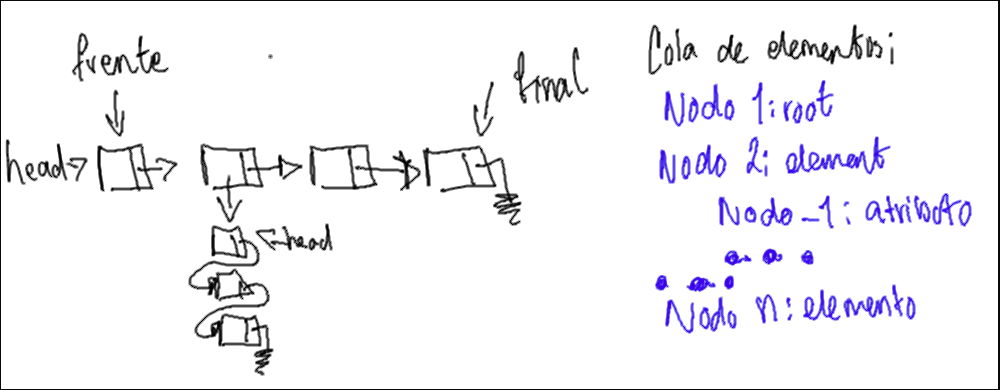
\includegraphics[width=0.9\linewidth]{boceto.png}
  \caption{superficie con traza}
\end{figure}

\end{sloppypar}
\end{document}

